\section{La hidrografía de España}

\subsection{Características de los ríos españoles}

Los ríos españoles (Figura \ref{fig:rios-espana}) se caracterizan por tener escaso caudal, régimen irregular y ser relativamente cortos. Solo cinco superan los 500 km de longitud. Mar Cantábrico Se distribuyen en tres vertientes hidrográficas de acuerdo con el océano o mar en el que desembocan.

\begin{figure}[!ht]
    \centering
    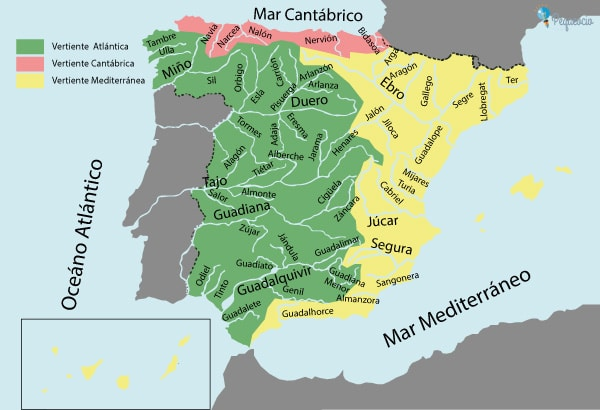
\includegraphics[width=0.7\linewidth]{Tema2/08_Rios-espana.jpg}
    \caption{Ríos de España}
    \label{fig:rios-espana}
\end{figure}

\subsection{Vertientes hidrográficas}

\subsubsection{Los ríos de la vertiente cantábrica}

Los ríos de esta vertiente \textbf{desembocan en el mar Cantábrico}. Son cortos, porque nacen en montañas próximas al mar, y caudalosos y de régimen regular, debido a las abundantes precipitaciones que reciben todo el año.

\vspace{3mm}
Los principales, de oeste a este, son: Eo, Navia, Nalón, con su afluente Narcea, Sella, Besaya, Saja, Pas, Nervión, Deva y Bidasoa.

\subsubsection{Los ríos de la vertiente atlántica}

Los ríos de esta vertiente \textbf{desembocan en el océano Atlántico}. Se diferencian dos tipos: los ríos gallegos y los que recorren la Meseta y la depresión del Guadalquivir.

\begin{itemize}
    \item Los ríos gallegos son cortos, caudalosos y regulares. Los más importantes son: Eume, Tambre, Ulla y Miño, con su afluente, el Sil.
    \item Los ríos de la Meseta son largos, caudalosos y de régimen irregular. Nacen en montañas alejadas del mar y solo reciben lluvias en otoño y primavera. Los principales son: Duero, Tajo, Guadiana y Guadalquivir.
\end{itemize}

\subsubsection{Los ríos de la vertiente mediterránea}

Los ríos de esta vertiente \textbf{desembocan en el mar Mediterráneo}. Se clasifican en ríos de las zonas este y sur.

\begin{itemize}
    \item Los ríos de la zona este son poco caudalosos, muy irregulares y de longitud variada, excepto el Ebro y el Ter. Destacan por importancia los ríos Ebro, que es el más caudaloso de España, Ter, Llobregat, Júcar y Segura.
    \item Los ríos de la zona sur son cortos, de caudal muy escaso y de régimen irregular, debido a las escasas precipitaciones. Los principales son, de oeste a este: Guadiaro, Guadalhorce, Guadalfeo, Andarax y Almanzora.
\end{itemize}

\subsection{La hidrografía de los archipiélagos}

En los archipiélagos balear y canario no hay ríos permanentes debido a la escasez de precipitaciones. Cuando llueve se forman torrentes, en Baleares, y barrancos, en Canarias.